\chapter{Perancangan}
\label{chap: perancangan}
	
	Pada bab ini akan dijelaskan mengenai perancangan aplikasi yang dibangun meliputi perancangan kelas, \textit{routes}, \textit{controllers}, \textit{models}, perancangan antarmuka.
	
	\section{Routes}
	\label{sec: routes}
	
	\textit{Routes} merupakan bagian dari \textit{codeigniter} untuk melakukan pemetaan terhadap lokasi \textit{file controllers} dari aplikasi. Di dalam \textit{routes} terdapat fungsi-fungsi khusus yang diperlukan untuk menjalankan aplikasi, seperti melakukan pemanggilan \textit{file controller} yang digunakan sebagai controller dasar pada aplikasi.

	\section{Controllers}
	\label{sec: controllers}
	
	\textit{Controller} terdiri dari sebuah kelas yang dinamakan "C\_Skripsi". Keseluruhan aktivitas dari sistem informasi penilaian skripsi diatur oleh kelas ini. Controller adalah \textit{file} yang mengatur hubungan antara \textit{file model} dan \textit{file view} pada sistem usulan yang akan dibangun. Fungsi untuk mengubah \textit{data} masukan yang akan diproses oleh \textit{file model} juga diatur di dalam \textit{file controller} ini.
	
	
	\section{Models}
	\label{sec: models}
	
	\textit{Models} mempunyai fungsi menghubungkan \textit{views} dan \textit{controllers} pada basis data. Pada penggunaan \textit{codeigniter}, \textit{model} dibuat dengan sangat sederhana. Pada sistem usulan yang dibangun, \textit{file model} berfungsi untuk melakukan fungsi \textit{insert data} dari \textit{file view} kepada basis data. \textit{Parameter insert data} yaitu data masukan didapatkan dari fungsi yang terdapat pada \textit{file controller}.
	
	\section{Perancangan Basis Data}
	\label{sec: perancanganDatabase}
	
	Berdasarkan analisis basis data pada bab \ref{sub: analisisDatabase}, maka dibuat tabel basis data.
	\begin{table}[H]
	\centering
	\caption{Tabel Perancangan Basis Data}
	\begin{tabular}{| m{0.75cm} | m{7cm} | m{3cm} |}
		\hline
		No & Nama Tabel & Jenis Data\\
		\hline
		1 & \underline{id} & int(11)\\
		\hline
		2 & tahun & year(4)\\
		\hline
		3 & semester & int(1)\\
		\hline
		4 & npm & varchar(10)\\
		\hline
		5 & nama & varchar(256)\\
		\hline
		6 & judul & varchar(256)\\
		\hline
		7 & namaPembimbing & varchar(256)\\
		\hline
		8 & namaPembimbingPendamping & varchar(256)\\
		\hline
		9 & namaKetuaTimPenguji & varchar(256)\\
		\hline
		10 & namaAnggotaTimPenguji & varchar(256)\\
		\hline
		11 & bobotKetuaTimPenguji & int(2)\\
		\hline
		12 & bobotAnggotaTimPenguji & int(2)\\
		\hline
		13 & bobotPembimbing & int(2)\\
		\hline
		14 & nilaiKoordinatorSkripsi & float\\
		\hline
		15 & bobotKoordinatorSkripsi & int(2)\\
		\hline
		16 & bobotTataTulisLaporanAnggota & int(2)\\
		\hline
		17 & bobotKelengkapanMateriAnggota & int(2)\\
		\hline
		18 & bobotPenguasaanMateriAnggota & int(2)\\
		\hline
		19 & bobotPresentasiAnggota & int(2)\\
		\hline
		20 & bobotPencapaianTujuanAnggota & int(2)\\
		\hline
		21 & bobotTataTulisLaporanKetua & int(2)\\
		\hline
		22 & bobotKelengkapanMateriKetua & int(2)\\
		\hline
		23 & bobotPenguasaanMateriKetua & int(2)\\
		\hline
		24 & bobotPresentasiKetua & int(2)\\
		\hline
		25 & bobotPencapaianTujuanKetua & int(2)\\
		\hline
	\end{tabular}
\end{table}
\begin{table}[H]
\centering
	\begin{tabular}{| m{0.75cm} | m{7cm} | m{3cm} |}
	\hline
		26 & bobotTataTulisLaporanPembimbing & int(2)\\
		\hline
		27 & bobotKelengkapanMateriPembimbing & int(2)\\
		\hline
		28 & bobotPenguasaanMateriPembimbing & int(2)\\
		\hline
		29 & prosesBimbinganPembimbing & int(2)\\
		\hline
		30 & nilaiAkhirMahasiswa & float\\
		\hline
		\end{tabular}
	\end{table}
	
	\section{Perancangan Tampilan}
	\label{sec: perancanganTampilan}
	
	Tampilan pada sistem informasi penilaian skripsi haruslah dibuat semirip mungkin dengan form penilaian skripsi yang sudah ada seperti pada lampiran gambar \ref{fig: skripsiAsli} dan gambar \ref{fig: rekapAsli}.
	
	Perbedaan yang akan ditampilkan adalah dengan adanya otomatisasi penghitungan nilai sesuai dengan bobot yang diberikan kepada penilai. Hal ini akan memberikan kemudahan penilai untuk melakukan penilaian.
	
	Gambar \ref{fig:beritaacara} adalah bayangan awal tampilan untuk sistem informasi penilaian skripsi lembar berita acara sidang skripsi.
	\begin{figure}[H]
		\centering
		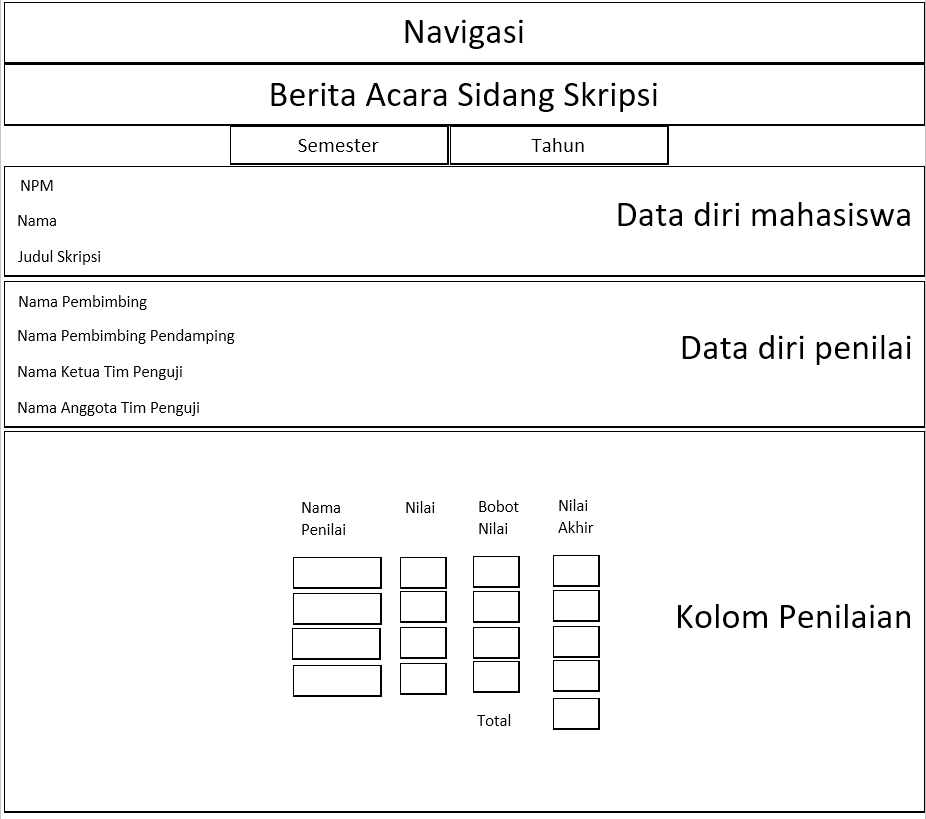
\includegraphics[scale=0.75]{Gambar/beritaacara}
		\caption{Perkiraan Tampilan Lembar Berita Acara Sidang Skripsi}
		\label{fig:beritaacara}
	\end{figure}
	
	Keterangan Gambar\ref{fig:beritaacara}.
	\begin{enumerate}
		\item Tempat navigasi untuk berpindah halaman
		\item Judul formulir penilaian
		\item Data diri mahasiswa (nama, NPM, judul skripsi)
		\item Data diri penilai (nama ketua tim penguji, anggota tim penguji, pembimbing, dan pembimbing pendamping)
		\item Penanda kategori penilaian
		\item Kotak masukan nilai per kategori (otomatis)
		\item Bobot nilai yang dimiliki kategori (\textit{default})
		\item Nilai hasil perhitungan masukan dengan bobot (otomatis)
	\end{enumerate}
	
	Gambar \ref{fig:rekapitulasi} adalah bayangan awal tampilan untuk sistem informasi penilaian skripsi lembar rekapitulasi ketua tim penguji, anggota tim penguji, dan pembimbing.
	\begin{figure}[H]
		\centering
		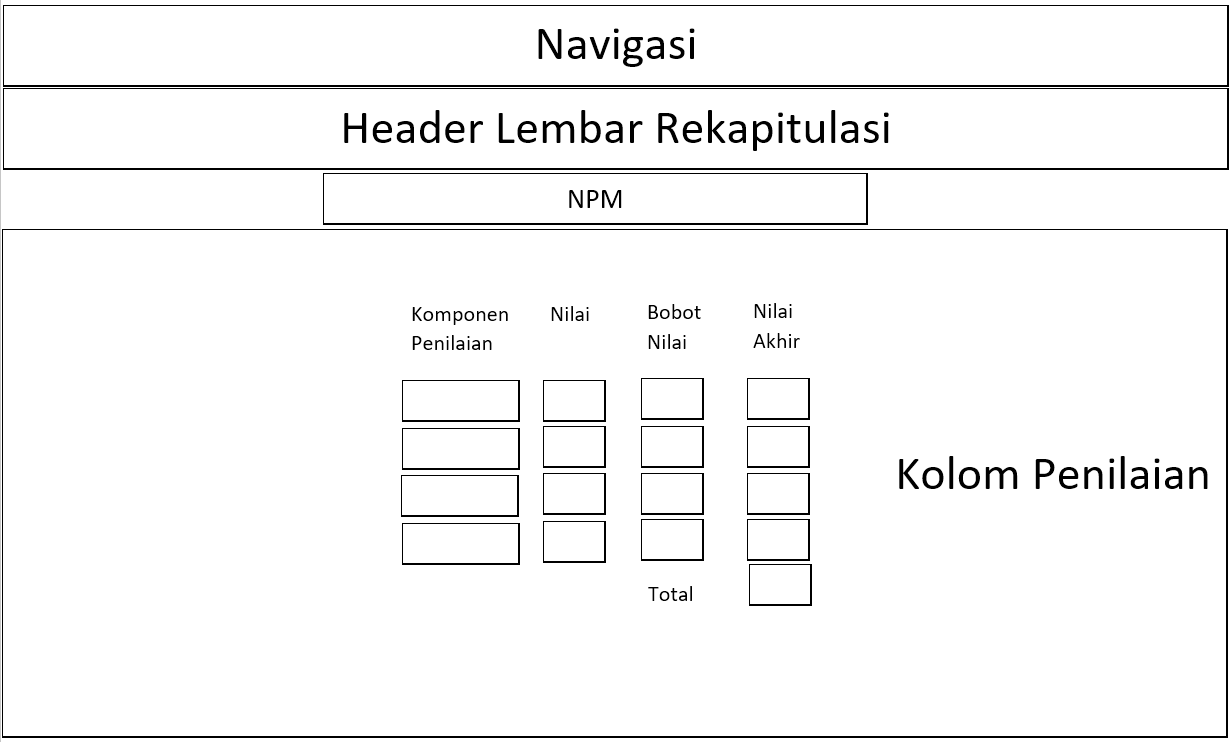
\includegraphics[scale=0.5]{Gambar/rekapitulasi}
		\caption{Perkiraan Tampilan Lembar Rekapitulasi}
		\label{fig:rekapitulasi}
	\end{figure}
Keterangan Gambar \ref{fig:rekapitulasi}.
\begin{enumerate}
	\item Tempat navigasi untuk berpindah halaman
	\item Judul formulir penilaian
	\item NPM mahasiswa (otomatis)
	\item Penanda kategori penilaian
	\item Kotak masukan nilai per kategori (masukan)
	\item Bobot nilai yang dimiliki kategori (\textit{default})
	\item Nilai hasil perhitungan masukan dengan bobot (otomatis)
\end{enumerate}